\documentclass[12pt,a4paper]{article}
\usepackage{physics}
\usepackage{amssymb, amsmath}
\usepackage{subcaption}
\newcommand{\activity}{Activity 15 -- Expectation Maximization}
\input{spp.dat}

\begin{document}

\title{\TitleFont \activity}
\author[ ]{\textbf{Kenneth V. Domingo} \\
2015--03116 \\
App Physics 186, 1\textsuperscript{st} Semester, A.Y. 2019--20}
\affil[ ]{\corremail{kvdomingo@up.edu.ph} }

\maketitle
\thispagestyle{titlestyle}

\section*{Results and Discussion}
\setcounter{section}{1}

For this activity \cite{soriano}, I used the separated banana, apple, and orange feature data from a previous activity. The fruits form clear clusters in $a^*-b^*$ feature space and is suitable for this activity. Figure \ref{fig:ab-space} shows the clustering of the fruit data. 

\begin{figure}[htb]
	\centering
	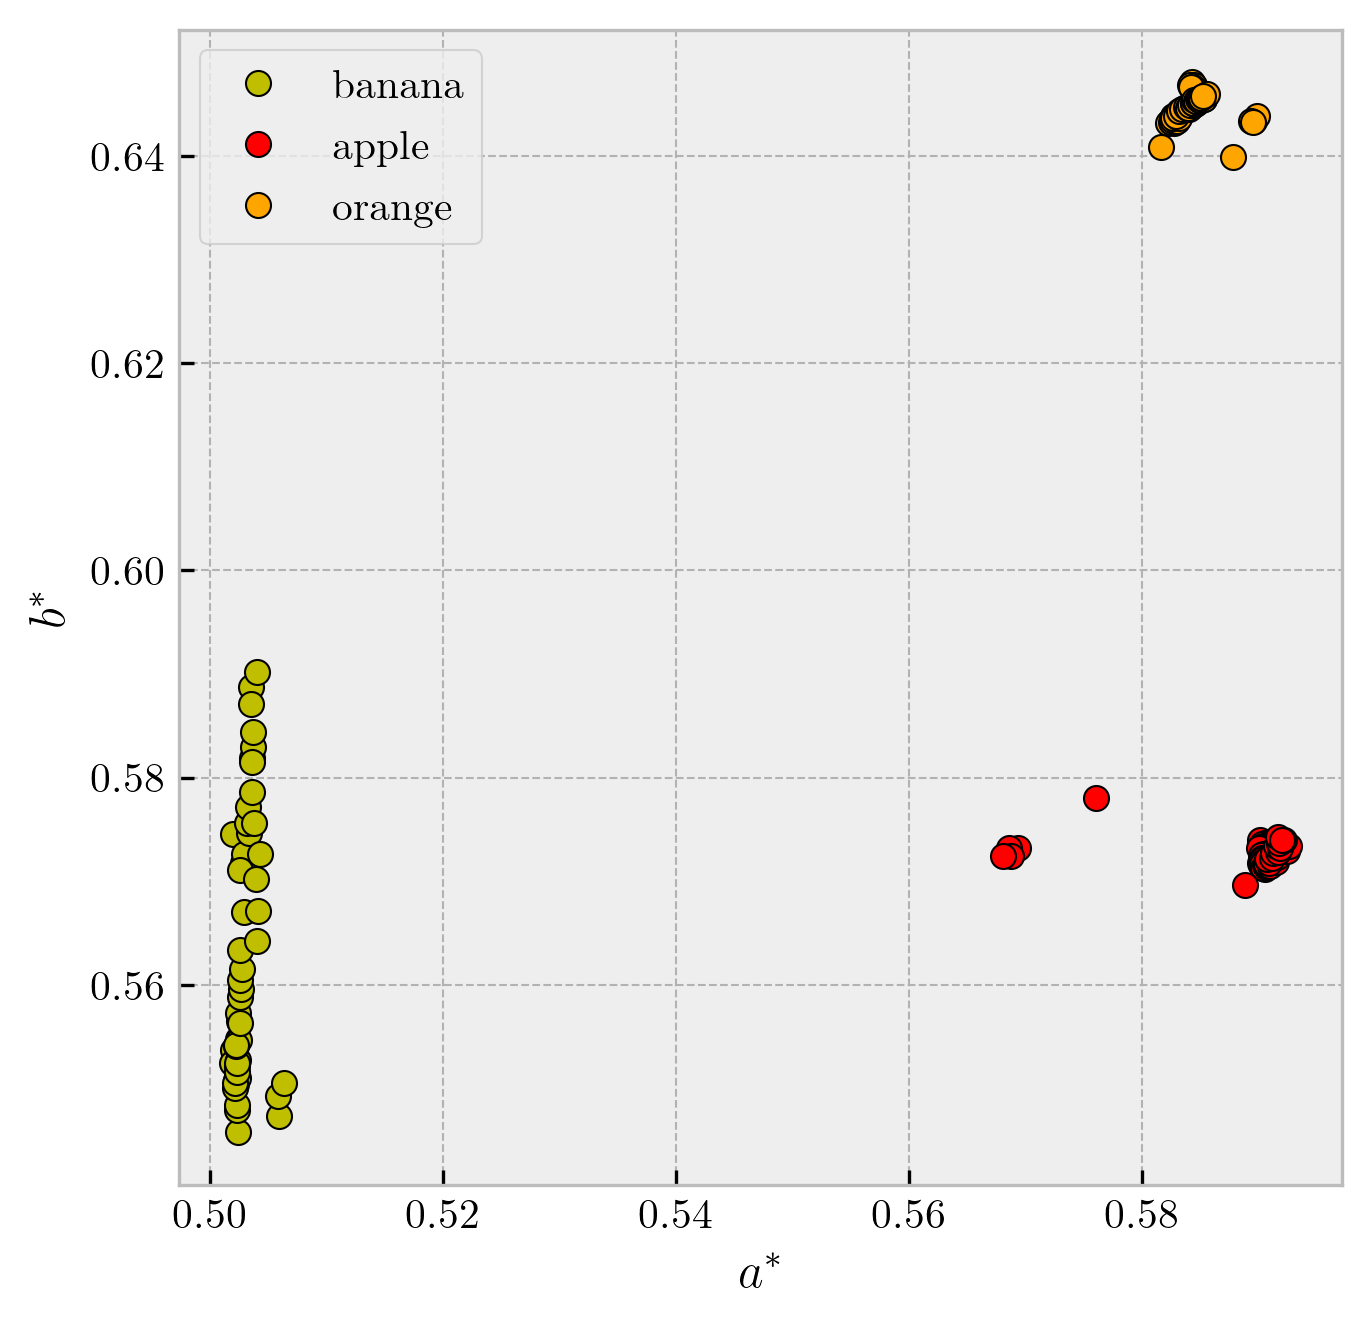
\includegraphics[width=0.7\textwidth]{ab-space.png}
	\caption{$a^*-b^*$ feature space of fruit data.}
	\label{fig:ab-space}
\end{figure}

Since we are working only with two dimensions (two features), we assume a 2D Gaussian distribution, given by

\begin{equation}
	p_l \qty(\vec{x} | \bm\mu_l, \bm\Sigma_l) = \frac{1}{2\pi \abs{\bm\Sigma_l}^{1/2}} \exp[-\frac{1}{2} \qty(\vec{x} - \bm\mu_l)^\top \bm\Sigma_l^{-1} \qty(\vec{x} - \bm\mu_l)]
\end{equation}

In the interest of computational efficiency, we define an intermediate matrix $\bm\omega$ whose elements are given by

\begin{equation}
	\omega_{li} = p_l \qty(\vec{x}_i | \bm\mu_l, \bm\Sigma_l)
\end{equation}

\noindent which are used throughout one entire iteration, in order to avoid redundant calculation of exponentials and matrix inversions. We then iterate with the update rules

\begin{align}
	P_l^\prime &= \frac{1}{N} \sum_{i=1}^N P \qty(l | \vec{x}_i, \bm\Theta^g) \\
	\bm\mu_l^\prime &= \frac{\sum_{i=1}^N \vec{x}_i P \qty(l | \vec{x}_i, \bm\Theta^g)}{\sum_{i=1}^N P \qty(l | \vec{x}_i, \bm\Theta^g)} \\
	\bm\Sigma_l^\prime &= \frac{\sum_{i=1}^N P \qty(l | \vec{x}_i, \bm\Theta^g) \qty(\vec{x}_i - \bm\mu_l^\prime) \qty(\vec{x}_i - \bm\mu_l^\prime)^\top}{\sum_{i=1}^N P \qty(l | \vec{x}_i \bm\Theta^g)}
\end{align}

\noindent until the log-likelihood goes above some pre-set value. The log-likelihood is given by

\begin{equation}
	L = \ln \qty[\sum_i \sum_l P_l^\prime p_l \qty(\vec{x}_i | \bm\mu_l, \bm\Sigma_l)]
\end{equation}

\noindent The PDF shown in Fig. \ref{fig:pdf} is obtained at an average of 31 epochs.

\begin{figure}[htb]
	\centering
	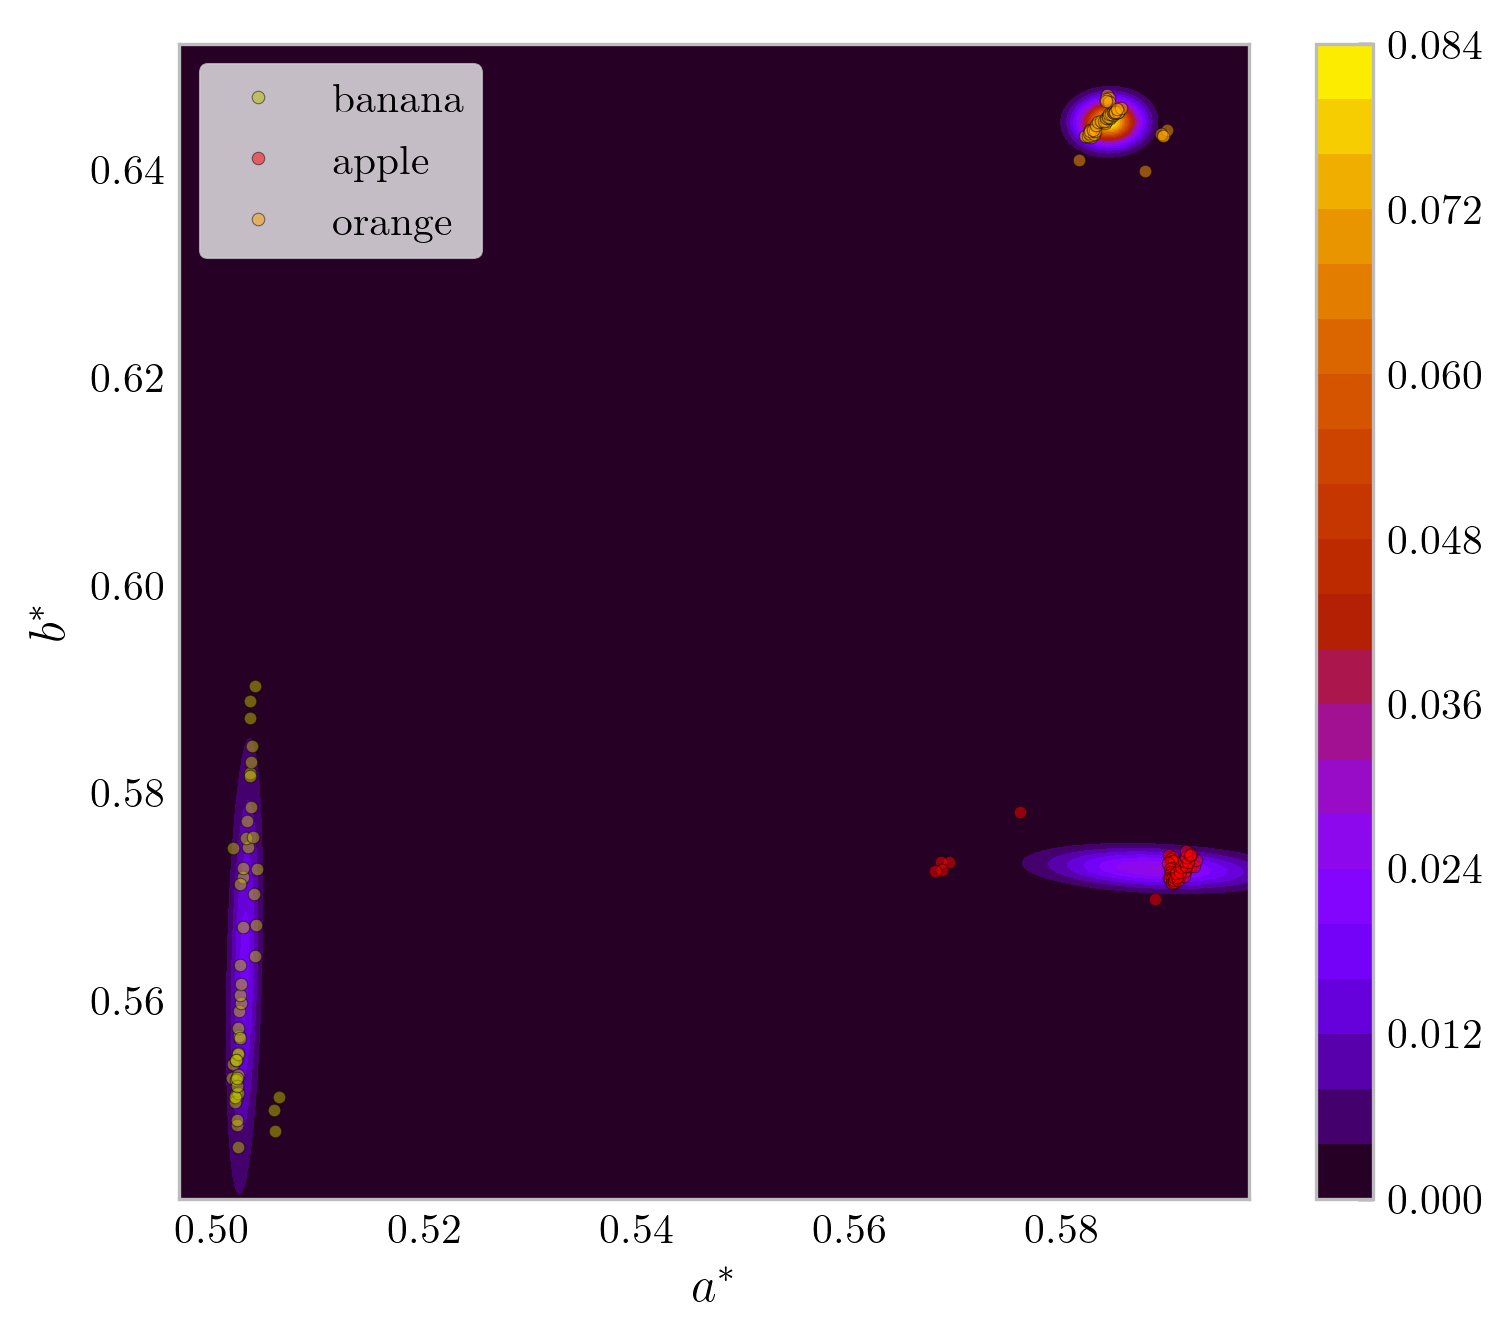
\includegraphics[width=0.7\textwidth]{em-feature-space.png}
	\caption{Estimated PDF in the $a^*b^*$ feature space of bananas, apples, and oranges.}
	\label{fig:pdf}
\end{figure}

\clearpage
\begin{table}[!htb]
	\centering
	\caption{Self-evaluation.}
	\begin{tabular}{||r|c||}
		\hline
		Technical correctness & 5 \\ \hline
		Quality of presentation & 5 \\ \hline
		Initiative & 0 \\ \hline
		\textbf{TOTAL} & \textbf{10} \\ \hline
	\end{tabular}
	\label{tab:self-eval}
\end{table}

\bibliographystyle{spp-bst}
\bibliography{biblio}

\end{document}